\subsection{The Rise of Mobile Applications }
Mobile applications have become integral to daily life globally, revolutionizing various sectors such as healthcare, education, finance, and entertainment. The rise of mobile applications has significantly impacted society, leading to increased dependence on mobile technologies. Integrating information and communication technologies (ICTs) like mobile phones and the Internet with financial services has given rise to new forms of digital finance, including mobile payments, online credit, and intelligent investment advice \cite{li2022impact}. This integration has transformed financial services and facilitated access to formal financial services for underserved populations, such as smallholder farmers \cite{omar2022predictors}.
\par
The rapid growth of the mobile app market is evident in the increasing adoption of mobile payment systems. Mobile payment systems have increased employment and income for family members, particularly benefiting low-income and rural households \cite{wang2020mobile}. Moreover, the development of financial innovations like mobile payments and AI-based credit scoring systems has immense potential to increase financial inclusion, enabling the unbanked population to participate actively in financial markets \cite{rybakovas2022financial}.
\par
In addition to finance, mobile applications have also played a crucial role in healthcare. Mobile smartphone applications provide a unique platform to promote the utilization of evidence-based skills, especially in areas like substance use treatment \cite{dahne2015smartphone}. Furthermore, the education sector has witnessed a transformation with the increasing use of mobile applications. The study indicates that mobile banking, a mobile application, has provided smallholder farmers access to formal financial services like deposits and loans, which previously needed to be improved \cite{omar2022predictors}.
\par
Entertainment is another sector significantly impacted by mobile applications. Note that mobile phones, through various entertainment apps, compete for limited attention with social networks, videos, games, and other types of entertainment \cite{zhang2023entertainment}. This competition for attention underscores the widespread use and popularity of entertainment apps on mobile devices.
\begin{figure}[htbp]
    \centering
    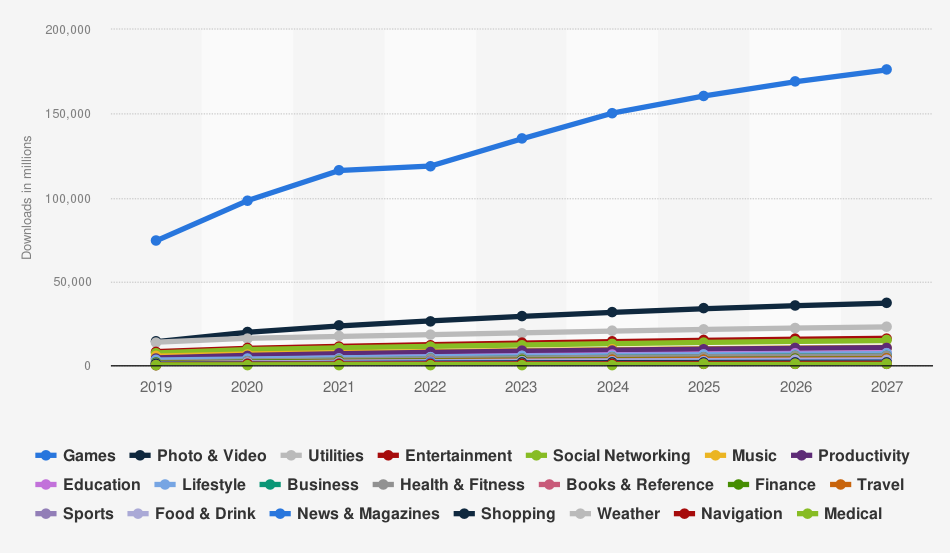
\includegraphics[scale = 0.45]{img/num_of_downloads.png}
    \caption{Number of mobile app downloads worldwide from 2019 to 2027, by segment(in million downloads) \cite{statista2023}}
    \label{fig:num_of_downloads}
\end{figure}
\par
The Figure \ref*{fig:num_of_downloads} clearly illustrates a continuous and significant growth in mobile application downloads across all sectors, with projections reaching up to 176.1 billion downloads in the Games segment by 2027. This trend, consistent throughout the forecast period from 2019 to 2027, emphasizes the expanding role and importance of mobile applications in daily life and various industries.
\par
The statistics and trends in mobile application usage globally reflect a trajectory of growth and innovation. The increasing reliance on mobile technologies across sectors underscores the transformative impact of mobile applications on society, paving the way for enhanced accessibility, efficiency, and convenience in various aspects of daily life. 
\subsection{Evolution of Mobile Development Approaches}
The evolution of mobile app development has seen significant advancements from early platforms to the modern ecosystems of Android and iOS. Initially, Java dominated Android development, offering a robust and versatile language for creating mobile applications. However, the introduction of Kotlin by JetBrains marked a pivotal moment in Android development. Kotlin, with its concise syntax, enhanced safety features, and seamless interoperability with Java, quickly gained popularity among developers. Google recognized the potential of Kotlin and endorsed it as a preferred language for Android app development, leading to widespread adoption within the Android community \cite{zhang2023entertainment}.
\par
Moreover, the emergence of cross-platform frameworks has revolutionized mobile app development by enabling developers to write code once and deploy it across multiple platforms. Flutter, developed by Google, has gained prominence among these frameworks for its efficiency and flexibility in building high-quality native interfaces. Flutter allows for fast development, expressive UIs, and native performance, making it popular for developers aiming to create visually appealing and responsive applications.
\par
Adopting Kotlin and Flutter signifies a shift towards more efficient and streamlined mobile app development practices. Kotlin's modern features and seamless integration with existing Java codebases have simplified the development process. At the same time, Flutter's cross-platform capabilities have empowered developers to create visually rich and performant applications across different operating systems. These advancements highlight the continuous evolution of mobile development approaches, emphasizing the importance of innovation and adaptability in the ever-changing landscape of mobile technology.
\subsection{Importance of Choosing the Right Development Approach}
Choosing between native development and cross-platform frameworks is a strategic decision that goes beyond technical considerations and impacts the success of a mobile application. Native development offers optimized performance and better access to device-specific features, ensuring high user satisfaction. On the other hand, cross-platform frameworks provide advantages such as faster rollout and cost-effectiveness. The decision between these approaches has implications for app performance, maintainability, and overall user experience, making selecting the appropriate development approach crucial.
\par
Native development, often associated with languages like Java for Android and Swift for iOS, allows developers to leverage platform-specific features and functionalities, resulting in high-performance applications tailored to each operating system. However, the development time and cost for native apps can be higher due to the need to write separate codebases for different platforms.
\par
In contrast, cross-platform frameworks like Flutter, React Native, and Xamarin enable developers to write code once and deploy it across multiple platforms, reducing development time and costs. While cross-platform development offers advantages in terms of efficiency and cost-effectiveness, there may be trade-offs in terms of performance optimization and access to certain platform-specific features.
\par
The study emphasizes the importance of well-defined technical requirements and specifications in selecting a cross-platform framework or development approach. Specific cross-platform frameworks can perform equally or even better than native in particular metrics, highlighting the need for a deliberate and informed decision-making process \cite{biorn2020empirical}.
\par
Ultimately, the choice between native development and cross-platform frameworks should align with the mobile application’s project requirements, budget constraints, and long-term goals. Understanding the implications of each approach on app performance, maintainability, and user satisfaction is essential for making an informed decision that maximizes the mobile application's success.
\subsection{Comparative Analysis: Java, Kotlin, and Flutter }
Java and Kotlin have been long-standing choices for native Android app development, with Java being the traditional standard and Kotlin emerging as a modern alternative. Java, known for its robustness and extensive ecosystem, has been widely used for Android development \cite{wasilewski2021comparison}. On the other hand, Kotlin, being interoperable with Java, offers a more concise syntax and additional safety features, enhancing code readability and reducing bugs \cite{ardito2020effectiveness}. The transition from Java to Kotlin has been notable, with Google endorsing Kotlin as the preferred language for Android app development \cite{coppola2019characterizing}.
\par
In contrast, Flutter, utilizing Dart, has gained attention for its cross-platform capabilities. It offers a single codebase for both Android and iOS platforms. This approach dramatically simplifies development and reduces maintenance costs \cite{prasetia2023development}. Flutter has been recognized as a framework that streamlines the development of cross-platform applications, providing efficiency and cost-effectiveness \cite{Meiller_2022}.
\par
The comparative analysis of Java, Kotlin, and Flutter reveals distinct advantages and challenges associated with each technology. Java and Kotlin excel in native Android development, with Kotlin offering modern features and improved safety. On the other hand, Flutter stands out for its cross-platform capabilities, enabling developers to create applications for multiple platforms with a single codebase. Understanding the strengths and limitations of each technology is essential for making informed decisions in mobile app development.
\subsection{Critical Role of Code Quality}
The quality of code is a vital component of software development, as it has a significant impact on the performance, scalability, and maintainability of applications. Key indicators of code quality include identifying code smells, which are patterns in the code that may indicate potential issues, and assessing the overall complexity of the codebase. Although code smells may not immediately affect the program's functionality, they can increase the risk of bugs or failures down the line and make maintenance more complex. Thus, it is critical to evaluate and address these smells to ensure the long-term quality and sustainability of software applications, as noted by Banker et al. \cite{banker1998software}.
\par
In software development, code quality is closely tied to developers' skills and capabilities. Research has shown that content software developers are more productive and effective in problem-solving. Psychological measurements in empirical software engineering have emphasized the significance of factors such as high analytical problem-solving skills and creativity in the software construction process, highlighting the role of developer well-being in software quality and productivity \cite{graziotin2014happy}.
\par
Efforts to enhance software quality often involve methodologies like the Capability Maturity Model (CMM), which aims to improve software development processes to deliver high-quality software within budget and planned cycle time. Adopting structured approaches like CMM can result in improved software quality, reduced defects, and increased efficiency in the software development lifecycle \cite{agrawal2007software}.
\par
Analyzing code quality across different programming languages and frameworks, such as Java, Kotlin, and Flutter, can offer valuable insights into the impact of development choices on software quality. Leveraging tools like SonarQube for evaluating and comparing code quality metrics can provide a quantitative basis for assessing the effectiveness of development practices and identifying areas for improvement. Developers can enhance software applications' overall quality and reliability by systematically analyzing code quality indicators and addressing issues such as code smells and complexity, improving user experiences and long-term success \cite{graziotin2018happens}.
\subsection{Research Gap}
Despite the critical role of mobile applications in various sectors and the rapid evolution of development technologies, there remains a significant gap in empirical research regarding the comparative analysis of mobile development approaches, particularly regarding their impact on code quality. Most existing studies focus on individual aspects of development, such as usability, performance, or developer preferences. Still, few comprehensively evaluate how different programming languages and frameworks—like Java, Kotlin, and Flutter—affect code's overall quality and maintainability.
\par
Current literature extensively discusses the features and benefits of Kotlin and Flutter, noting their potential to streamline the development process and enhance code safety and maintainability. However, more systematic empirical studies need to quantify the impact of these modern languages and frameworks on code quality in real-world development scenarios. This includes a detailed analysis of code smells, which are subtle indicators of potential future problems or technical debt that might not currently affect an application's functionality but could lead to significant maintenance challenges.
\par
Furthermore, while tools like SonarQube offer capabilities to assess and compare code quality metrics across different environments, the practical application of these tools in comparative studies must be extensively documented in academic research. Studies that not only use these tools to gather data but also critically analyze this data to provide actionable insights into how specific characteristics of Java, Kotlin, and Flutter influence the maintainability, scalability, and efficiency of the development process are needed.
\par
This research aims to fill these gaps by conducting a rigorous comparative analysis of mobile applications developed in Java, Kotlin, and Flutter. It will evaluate various code quality metrics, such as the prevalence and severity of code smells and the overall complexity of the codebases, to determine the tangible impacts of choosing one technology over another. This study will provide empirical evidence to guide developers in selecting the most suitable programming language or framework for their projects based on quantifiable code quality and maintainability measures.
\par
By addressing this research gap, the study will contribute valuable insights to the field of software engineering, particularly mobile app development. It will enhance understanding of the practical implications of development tool choices on long-term application success and sustainability.
\subsection{Study Objectives and Research Questions}
The overarching objective of this thesis is to conduct a thorough empirical analysis to compare the impact of different mobile development approaches—specifically Java, Kotlin, and Flutter—on the quality and maintainability of mobile applications. This research is driven by the need to provide developers and stakeholders with data-driven insights that can guide their decisions regarding which development technologies to adopt, depending on specific project requirements and goals. 
\par
The choice of focusing on these specific technologies is substantiated by their prevalent use and perceived benefits within the development community. According to a 2022 developer survey, Flutter has emerged as the most popular cross-platform mobile framework. The survey reports that 46 percent of software developers used Flutter, highlighting its significant adoption. This statistic is particularly compelling, considering that approximately one-third of mobile developers utilize cross-platform technologies, while the remainder prefer native tools.
\begin{figure}[htbp]
    \centering
    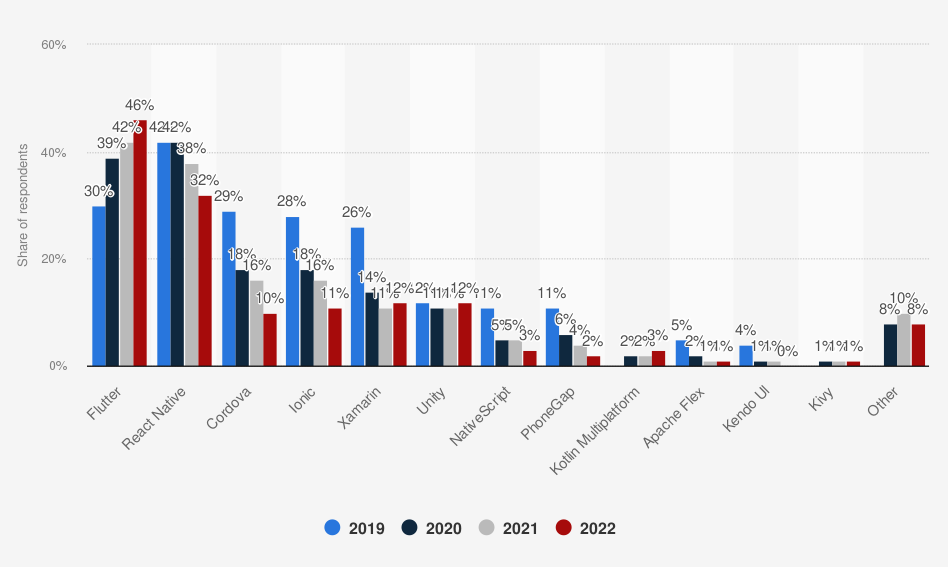
\includegraphics[scale = 0.45]{img/cross_platform-sts.png}
    \caption{Cross-platform mobile frameworks used by software developers worldwide from 2019 to 2022 \cite{jetbrains2022}}
    \label{fig:cross_platform-sts}
\end{figure}
\subsubsection*{Objectives}
\begin{enumerate}
    \item To evaluate the development efficiency of Java, Kotlin, and Dart. This includes measuring the time taken for development, the ease of implementation of features, and the integration of third-party services across the three languages.
    \item To analyze the maintainability of Java, Kotlin, and Dart applications.  Maintainability will be assessed by examining code complexity, readability, and the ability to adapt or extend the application with new features.
    \item This study aims to compare the code quality of applications developed using Java, Kotlin, and Dart(Flutter). Code quality will be evaluated based on the prevalence of code smells, adherence to coding standards, and the occurrence of bugs or issues during and after development.
    \item To provide recommendations on the choice of development approach based on empirical data: Based on the findings, the study aims to offer guidelines on selecting development approaches for different mobile app projects, considering factors like project size, complexity, and specific industry needs.
\end{enumerate}
\subsubsection*{Research Questions}
In pursuit of these objectives, the study will seek to answer the following research questions:
\begin{enumerate}
    \item Comparing the Efficiency and Resource Utilization of Java, Kotlin, and Dart: How does each technology stack up against one another regarding development efficiency, time, and resources required to create a fully operational mobile application? What are the implications of selecting each technology for the development process?
    \item Considering the Impact on Maintenance and Long-Term Code Quality: What are the consequences of choosing Java, Kotlin, or Dart on mobile application maintainability? How do code complexity, debugging ease, and change adaptability impact long-term maintenance and code quality in these development environments?
    \item Navigating Coding Challenges and Selection Criteria: How does each development approach—Java, Kotlin, or Dart—address prevalent coding challenges and quality issues, such as the frequency and severity of code smells? Based on these considerations, which development approach is most desirable for various mobile application projects? Considering project scope, performance requirements, and target platforms, what are the recommendations for language selection to optimize development outcomes?
\end{enumerate}
\subsection{Methodology, Significance, and Structure of Thesis}
A robust methodology has been adopted to achieve the research objectives outlined in this study, which involves developing a Kanban board application using three distinct programming environments: Java, Kotlin, and Flutter. The subsequent analysis of these applications will employ SonarQube, a sophisticated tool designed to assess metrics such as lines of code (LOC), code smells, and overall code quality. This method not only facilitates the collection of quantitative data concerning the efficiency and maintainability of each language but also provides qualitative insights into the coding experience. Such a dual-focused analysis enables a comprehensive understanding of the practical impacts of each development approach on project outcomes.
\par
The insights derived from this research are expected to be highly valuable for developers and project managers, guiding the selection of development tools and practices based on empirical evidence. By clearly delineating the strengths and weaknesses associated with Java, Kotlin, and Flutter, this study contributes to informed decision-making within the software development community. Such knowledge is crucial for enhancing app quality and developer satisfaction, and it is anticipated that the findings will encourage more efficient and effective development practices within the industry. The practical implications of this research are significant, offering potential improvements in development processes, resource allocation, and project management in mobile app development.
\par
This thesis is methodically structured into six comprehensive chapters, designed to guide the reader through the research process systematically:

\begin{itemize}
    \item \textbf{Introduction:} This opening chapter sets the stage by outlining the motivation for the study, the research gaps identified, and the objectives to be achieved.
    \item \textbf{Literature Review:} This section delves into a thorough review of existing research, discussing the theoretical frameworks and previous empirical studies relevant to mobile application development, mainly focusing on Java, Kotlin, and Dart(Flutter).
    \item \textbf{Methodology:} This section details the specific methods employed in the study, including the development processes for the Kanban board application in each programming environment and the analytical tools and criteria used to evaluate code quality. 
    \item \textbf{Results:} This paper presents a detailed account of the application development and analysis findings, offering a comparative perspective on the code quality metrics observed across the different programming environments.
    \item \textbf{Discussion:} This section interprets the results in the context of existing literature and discusses their implications for developers and the broader software development industry.
    \item \textbf{Conclusion and Recommendations:} This section summarizes the findings, discusses the study’s potential limitations, and offers recommendations for future research and practical applications in mobile app development.
\end{itemize}
